\thispagestyle{toancuabinone}
\pagestyle{toancuabi}
\everymath{\color{toancuabi}}
%\blfootnote{$^1$\color{toancuabi}Đại học Thăng Long.}
\graphicspath{{../toancuabi/pic/}}
\begingroup
\AddToShipoutPicture*{\put(0,616){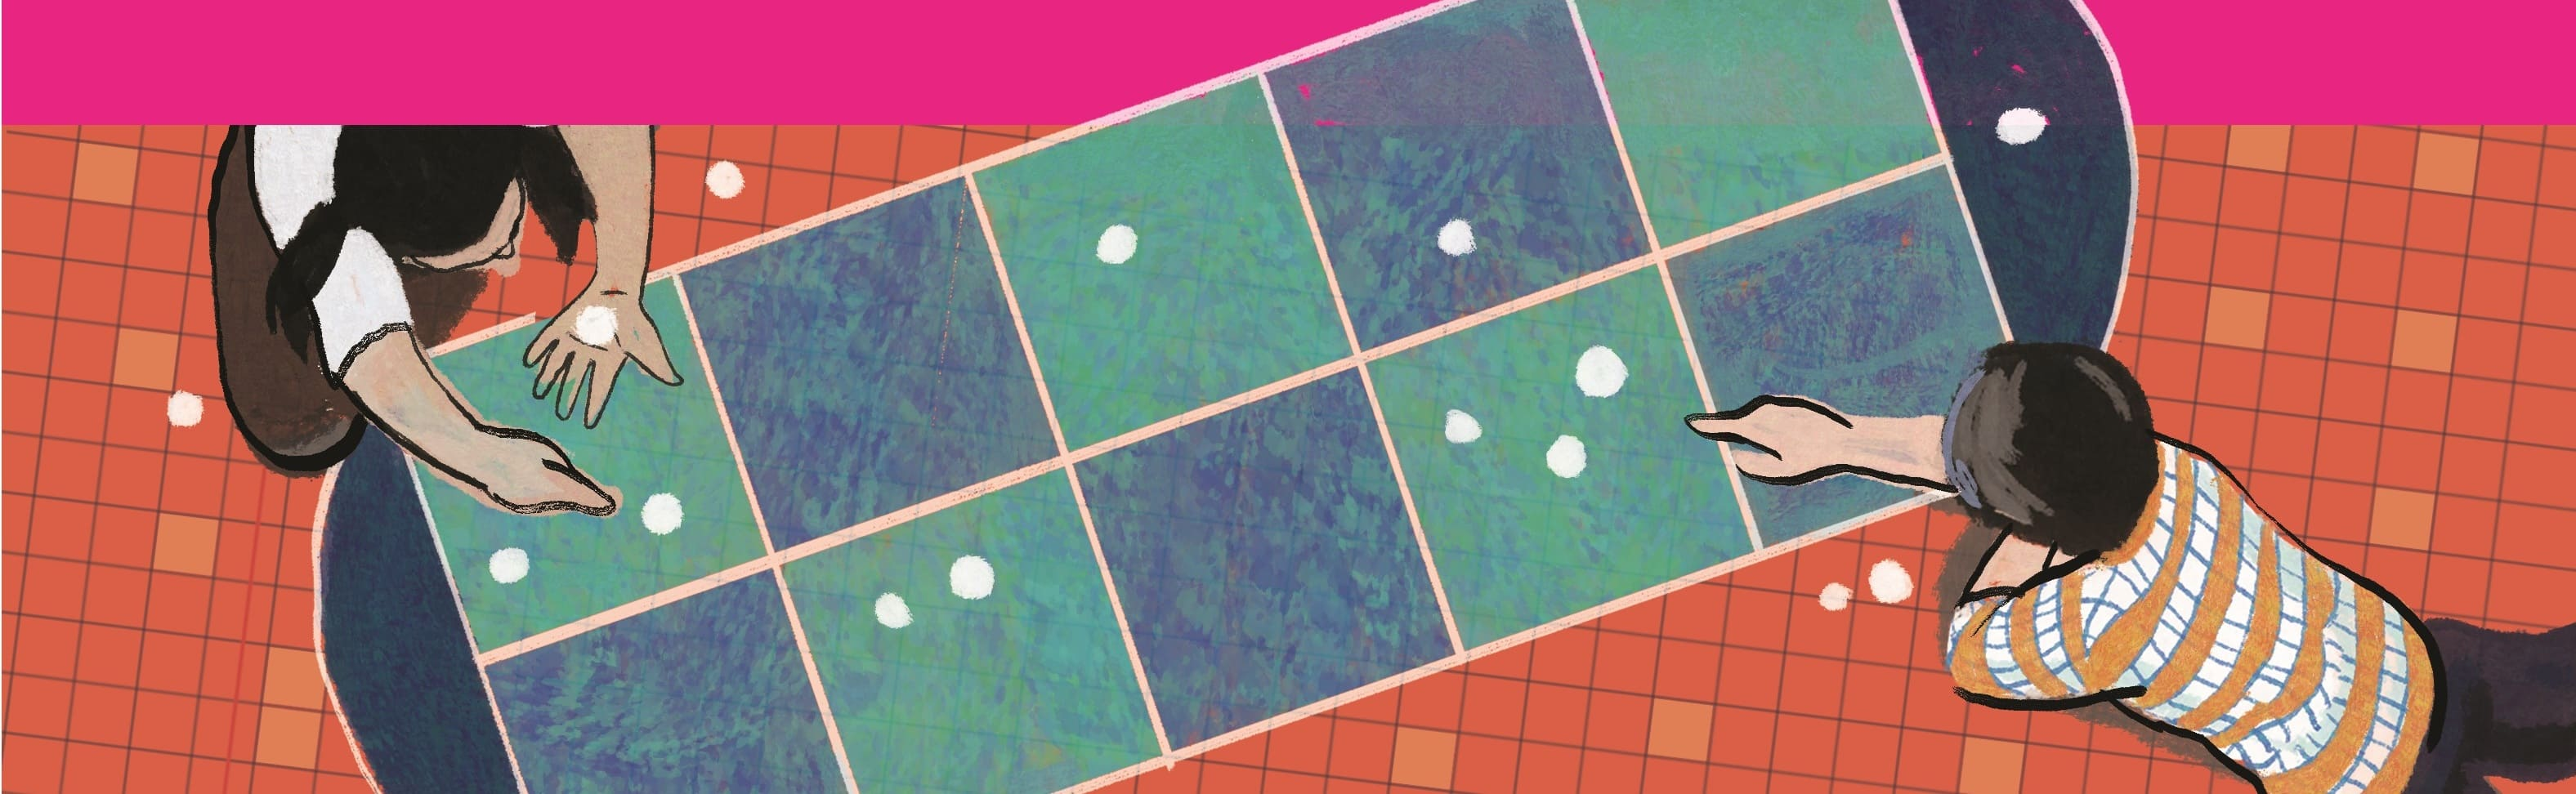
\includegraphics[width=19.3cm]{../bannertoancuabi}}}  
\AddToShipoutPicture*{\put(85,525){
\includegraphics[scale=1]{../tieude1.pdf}}} 
\centering
\endgroup

\vspace*{182pt}

\newpage
\begingroup
\thispagestyle{toancuabinone}
\blfootnote{$^1$\color{toancuabi}Ottawa, Canada.}
\AddToShipoutPicture*{\put(60,733){
\includegraphics[width=17.2cm]{../mathc.pdf}}}
%\AddToShipoutPicture*{\put(-2,733){
\includegraphics[width=17.2cm]{../mathl.pdf}}} 
\AddToShipoutPicture*{\put(189,675){
\includegraphics[scale=1]{../tieude4.pdf}}} 
\centering
\endgroup
\graphicspath{{../toancuabi/pic/}}
\vspace*{30pt}

\begin{multicols}{2}
	Below you see an example of \textit{family tree}.
	The circles denote female members and the triangles males.
	\begin{figure}[H]
		\vspace*{-5pt}
		\centering
		\captionsetup{labelformat= empty, justification=centering}
		\includegraphics[width= 0.75\linewidth]{hc-2022-2-3-15-1.pdf}
		\vspace*{-10pt}
	\end{figure}
	$A$ and $B$ are married, as are $F$ and $G,$ and $J$ and $K.$
	\vskip 0.1cm
	$B, C,$ and $D$ are siblings, as are $E$ and $F.$
	$E$ and $F$ are children of $A$ and $B.$
	\vskip 0.1cm
	Similarly, the parents of $I$ and $J$ are $F$ and $G.$
	$E$ is the father of $H.$
	\vskip 0.1cm
	In addition, $A$ is the grandmother of $H, I,$ and $J,$
	$F$ is the aunt of $H,$ and $C$ is the sister--in--law of $A.$
	\begin{figure}[H]
		\vspace*{-5pt}
		\centering
		\captionsetup{labelformat= empty, justification=centering}
		\includegraphics[width= 0.92\linewidth]{tree1}
%		\vspace*{-5pt}
	\end{figure}
	
	\vspace*{0.1pt}
	
	\vspace*{-7pt}
	\PIbox{
	{\color{toancuabi}\textbf{Example} (Who are who)\textbf{.}}
		Inspector Jade asked six children to briefly introduce their brothers, sisters,
		and first cousins (cousins who share a grandparent.)
		She had to match the name of the child to each numbered position in the family tree
		with the responses as below. Note that the relations given are in local languague.
		\textit{Do not try to guess the genders of the children from the names. It might lead you to the wrong way.}
	\vskip 0.1cm
	Response from Binh:
		\vskip 0.1cm
		$\circ$ I have three \textit{arawa}: Kim, Minh, Thao
		\vskip 0.1cm
		$\circ$ I have two \textit{surubu}: Oanh and Yen
		\vskip 0.1cm
		Response from Dinh:
		\vskip 0.1cm
		$\circ$ I have two \textit{surubu}: Oanh and Yen
		\vskip 0.1cm
		$\circ$ I have one \textit{ere}: Binh
		\vskip 0.1cm
		Response from Kim:
		\vskip 0.1cm
		$\circ$ I have one \textit{arawa}: Dinh
		\vskip 0.1cm
		$\circ$ I have one \textit{surubu}: Binh
		\vskip 0.1cm
		Response from Minh:
		\vskip 0.1cm
		$\circ$ I have one \textit{ere}: Yen
		\vskip 0.1cm
		$\circ$ I have two \textit{arawa}: Dinh and Thao
		\vskip 0.1cm
		Response from Thao:
		\vskip 0.1cm
		$\circ$ I have two \textit{surubu}: Yen and Binh
		\vskip 0.1cm
		$\circ$ I have two \textit{arawa}: Minh and Dinh}
	\begin{figure}[H]
		\vspace*{-5pt}
		\centering
		\captionsetup{labelformat= empty, justification=centering}
		\includegraphics[width= 1\linewidth]{hc-2022-2-3-15-2.pdf}
		\vspace*{-20pt}
	\end{figure}
	\textit{Solution.} From what Binh said, Binh has the same type of relations to three children.
		Thus, those cannot be Binh's sisters or brothers,
		and \textit{arawa} does not mean sister or brother.
		Only the child number $4$ or $5$ has three cousins in the same gender.
		\vskip 0.1cm
		Look at the cousins of the children $4$ or $5,$
		\textit{arawa} or \textit{suburu} rather related to the gender of the cousin
		than the gender of the cousin's father or the mother.
		Note that Binh is a \textit{suburu} to Kim and Kim is an \textit{arawa} to Binh.
		Thus, Binh and Kim are of opposite genders, so Binh is a girl.
		Hence, Binh is the girl number $4.$
		\vskip 0.1cm
		Therefore, Kim, Minh, and Thao are the children $1, 3,$ and $7,$
		and \textit{arawa} means \textit{male cousin(s).}
		Furthermore, Binh is a \textit{suburu} to Kim and Thao,
		in other words, she is a \textit{female cousin} to them.
		\vskip 0.1cm
		This means that Binh is not a \textit{suburu} to the boy $5.$
		Obviously, she is not an \textit{arawa} to anyone.
		Since she is an \textit{ere} to Dinh, Dinh must be her brother.
		Thus Dinh is the boy number $5.$
		\vskip 0.1cm
		Now, Thao must be the boy number $1$ because he has two female and two male cousins.
		That leaves Minh must be the boy number $3.$
		\vskip 0.1cm
		Yen is a \textit{ere} to Minh, so Yen is the girl number $2.$
		Finally, Oanh is the girl number $6.$
		\vskip 0.1cm
		The answer is $1-$Thao, $2-$Yen, $3-$Minh, $4-$Binh, $5-$Dinh, $6-$Oanh, $7-$Kim.
		\vskip 0.25cm
		\PIbox{
		\centerline{\textbf{\color{toancuabi}Vocabulary}}
		\vskip 0.1cm
		{\color{toancuabi}male}: nam
		\vskip 0.1cm
		{\color{toancuabi}female}: nữ
		\vskip 0.1cm
		{\color{toancuabi}family tree}: cây phả hệ 
		\vskip 0.1cm
		{\color{toancuabi}sibling}: anh/chị/em ruột 
		\vskip 0.1cm
		{\color{toancuabi}aunt}: cô, dì 
		\vskip 0.1cm
		{\color{toancuabi}sister--in--law}: chị/em dâu 
		\vskip 0.1cm
		{\color{toancuabi}cousin}: anh/chị/em họ 
		\vskip 0.1cm
		{\color{toancuabi}gender}: giới tính 
		}
\end{multicols}
\begin{figure}[H]
	\vspace*{-5pt}
	\centering
	\captionsetup{labelformat= empty, justification=centering}
	\includegraphics[width= 0.65\linewidth]{tree2}
	\vspace*{-5pt}
\end{figure}